\addcontentsline{toc}{part}{Cyatracking}
\part*{CyaTracking}
\section*{Qu'est-ce que c'est}
CyaTracking est un outil de statistiques permettant de recueillir diverses informations sur le trafic au sein d'une page de redirection. Une fois les informations collectées, l'utilisateur est redirigé vers une autre page.

\section*{Cahier des charges}

\subsection*{Formalistaion des besoins}

L'entreprise Cyanide possède un ensemble de pages boutique permettant l'achat des différents jeux qu'elle vend.
Elle désire pouvoir centraliser l'ensemble des adresses de boutique vers une seule et même page qui se chargera de rediriger l'utilisateur vers la bonne page.

De cet état de fait il est possible de réaliser un système d'affiliation en Cyanide et d'autres site internet qui s'ils décident de faire apparaitre sur leur page ou les réseaux sociaux un lien vers la page centrale de boutique, recevront un pourcentage sur chaque vente qui aurait transité par le lien de l'affilié.

L'URL choisie pour le lien respectera ce modèle-ci:


\textbf{http://store.cyanide-studio.com/?from=XXXXX\&lang=yy\_YY }

où:
\begin{itemize}
\item XXXXX: représente le numéro de l'affilié 
\item yy\_YY: indique la langue de la boutique à afficher 
\end{itemize}

Si les paramètres entrés sont incorrects ou inexistant il doit exister une adresse de redirection par défaut.

Un client devra permettre la visualisation des données des affiliés afin de connaître le nombre de redirection par affilié. La technologie pour celui-ci est libre.

\subsection*{Contraintes}
\begin{itemize}
\item Il est interdit de perdre une seule entrée.
\item Le script doit être suffisamment rapide pour permettre un trafic de pointe d'au moins 100 connections à la secondes. 
\item Les informations doivent être stockées en base de données MySQL.
\item L'intégralité du service doit tourner sur FreeBSD 10.0.
\item L'application doit être écrit en python version 2.7.
\item Respecter l'unité dans les services, la page de redirection devra tourner sur le serveur HTTP Apache 2.x+.
\end{itemize}

\newpage

\section*{Structure de l'application}

\begin{figure}[h!]
	\centering
	\includegraphics[scale=0.4]{images/cyatracking_network_scheme.png}
	\caption{Schéma réseau de l'ensemble de l'application}
\end{figure}

L'application était d'abord monolithique et situé sur le serveur de redirection, le traitement des informations est pour l'instant rapides mais dans l'avenir il est fort probable que ces processus soient plus long et complexes ce qui pourrait occasionner des ralentissements quant à la redirection de l'utilisateur. Il a donc été décider de distribuer les différentes fonctionnalités dans différents deux scripts indépendants qui communiquent entre via un socket de données. Le tout commandé par un troisième script de commande permettant d'influencer le comportement des scripts, car ceux-ci tournant en arrière plan, on ne dispose pas d'accès direct pour lancer des commandes.

\subsection*{Serveur de redirection}

Ce serveur possède un accès vers le reste du Web, sa tâche consiste à recueillir les différentes requêtes utilisateur via un serveur HTTP Apache qui a son tour transmettra la requête au script de redirection qui se chargera de réorienter l'utilisateur vers la page voulue.
Son rôle est aussi de transmettre les informations de l'utilisateur via socket au script de traitement. 

\subsection*{Serveur de traitement}
Son rôle est d'attendre des données en provenance du serveur de redirection et d'insérer les informations en base de données. Son fonctionnement sera expliqué en détails dans une partie qui lui est consacrée.


\subsection*{Poste de commande}
Celui-ci permet de donner des ordres aux deux autres scripts. Là aussi de plus amples détails seront donnés ultérieurement.

\subsection*{Base de données}
Il s'agit d'un serveur MySQL 5.5, il contient les différentes informations recueillies lors des redirections.

\underline{Remarque}:

Dans l'état actuel des choses le script de traitement, de redirection et de commande se trouvent sur le même serveur, mais rien n'empêche de les séparer.

\newpage

\section*{Script de redirection}
Comme il a été dit plus haut, le script doit tourner sur le serveur Apache pour cela deux solutions s'offrent à nous:
\begin{itemize}
\item \textbf{mod\_python}: ce plugin Apache permet d'interpréter un script python de la même manière que php-fpm pour le langage PHP. Il est livré avec un ensemble de module permettant de réaliser plus facilement un site web. Ce plugin est désormais déprécié il est recommandé de ne plus l'utiliser.
\item \textbf{wsgi} : le remplaçant de mod\_python, mais beaucoup plus léger s'appuyant sur l'utilisation de middlewares externes pour compléter les fonctionnalités manquantes.  
\end{itemize}
 
\subsection*{Structure minimale d'une application}

\begin{minted}{python}
def application(environ, start_response):
    """
    Simple Hello World wsgi app
    """
    output = "Hello World!"
    response_headers = [('Content-type', 'text/html'),('Content-Length', str(len("".join(output))))]
    start_response("200 OK", response_headers)
    return output
\end{minted}

Comme on peut le remarquer la structure de code minimale nécessaire à l'affichage d'une page est très restreint, seul 2 paramètres sont transmis à la fonction:
\begin{itemize}
	\item \textit{environ}: qui contient les différentes variables transmises par Apache, on y retrouve des informations telle que l'ip publique de la personne adressant la requête, le langage par défaut du navigateur, ainsi que le libellé du navigateur lui-même et le système d'exploitation. Ainsi que l'URL complète demandée.
	\item \textit{start\_response}: sert de lien entre le script python et le serveur Apache, il permet par exemple de modifier l'header et le statut de la réponse HTTP. 
\end{itemize}

\subsection*{Rediriger l'utilisateur}
Nous pouvons donc facilement effectuer les redirection en manipulant le champ \textbf{\textit{Location}} de l'header de la réponse HTTP.

\begin{minted}{python}
def redirect(start_response, to):
    response_headers = [('Content-type', 'text/html'),
                        ('Location',to),
                        ('Content-Length', "0")]
    start_response("303 See Other", response_headers)
    return [ ]
    
def application(environ, start_response):
    """
    Simple Hello World wsgi app
    """
    output = "Hello World!"
    return redirect(start_response, "http://somewhere.td")
\end{minted}

\newpage

Maintenant que nous possédons un moyen d'amener l'utilisateur sur une autre page, il s'agit de savoir où le rediriger. Pour cela il nous faut parser l'URL de requête via le module urlparse de python. Celui-ci nous permet de récupérer le chemin et les paramètres de l'URL simplement et même de parser les paramètres eux-même. Dans notre cas cela nous permet de récupérer les potentiels 
options lang et from contenus dans l'URL.

\subsubsection*{Configuration des redirections}
Afin d'apporter de la souplesse à l'application il a été décidé d'utiliser un fichier de configuration écrit en xml.

En voici la structure:


\begin{lstlisting}[language=XML]
<projects default-redirection="http://www.cyanide-studio.com">
    <project name="projet" default-redirection="http://store.cyanide-studio.com/project2" disable="1">
    </project>
    <project name="projet1" default-redirection="http://store.project1.com">
    </project>
    <project name="projet2" default-redirection="http://store.project2.com">
        <redirections>
            <redirection lang="en_US"><![CDATA[http://store.somewhere.com/?typnews=]]></redirection>
            <redirection lang="en_GB"><![CDATA[http://store.somewhere.com/?typnews=]]></redirection>
            <redirection lang=""><![CDATA[http://store.somewhere.com/?Langue=en_GB&typnews=]]></redirection>
            <redirection lang="fr_FR"><![CDATA[http://store.somewhere.com/?Langue=fr_FR&typnews=]]></redirection>
            <redirection lang="de_DE"><![CDATA[http://store.somewhere.com/?Langue=de_DE&typnews=]]></redirection>
            <redirection lang="es_ES"><![CDATA[http://store.somewhere.com/?Langue=es_ES&typnews=]]></redirection>
            <redirection lang="nl_NL"><![CDATA[http://store.somewhere.com/?Langue=nl_NL&typnews=]]></redirection>
            <redirection lang="it_IT"><![CDATA[http://store.somewhere.com/?Langue=it_IT&typnews=]]></redirection>
        </redirections>
    </project>
</projects>
\end{lstlisting}

\subsubsection*{Déterminer redirection}

La décision de la redirection se réalise sur plusieurs échelle:

Tout d'abord au niveau de l'application en elle-même, il est en effet possible d'indiquer une redirection par défaut globale, celle-ci est définie ligne 1.

Ensuite cette configuration peut spécifier pour chaque projet, on remarque d'ailleurs ici la possibilité de réaliser des alias entre les projets, comme c'est le cas pour le projet "projet" qui redirige vers le projet2, la requête est donc traité comme venant du projet 2.

Afin de rajouter de la granularité sur le choix de la langue de redirection chaque projet peut s'il le désire définir des redirections différentes par langues.

Par défaut, si aucun paramètre de langue n'existe dans la requête ou si celle-ci ne figure pas dans le fichier de configuration, alors la redirection ayant l'attribut lang="" sera utilisée.

Si une solution correcte de redirection n'est pas trouvée à l'étage courant on remonte au parent et ainsi de suite jusqu'à la redirection par défaut de l'application.


\subsubsection*{Le numéro d'affilié}

S'il est transmis le numéro d'affilié est contenu dans le paramètre \textit{from} de l'URL. Celui-ci doit-être un nombre. Dans le cas contraire un numéro d'affilié par défaut arbitrairement choisi comme étant le 99, sera  utilisé.

\subsubsection*{La gestion des alias}
Du fait que l'on fait rebondir l'utilisateur d'une page à une autre, il nous faut donc réécrire l'URL avant de la relancer pour traitement
Ceci est grandement facilité par urlparse qui nous permet de récupérer les paramètres de l'URL et de simplement les ajouter au lien de redirection.

\newpage

L'ensemble de l'algorithme de redirection est détaillé ci-dessous:

\begin{figure}[h!]
	\centering
	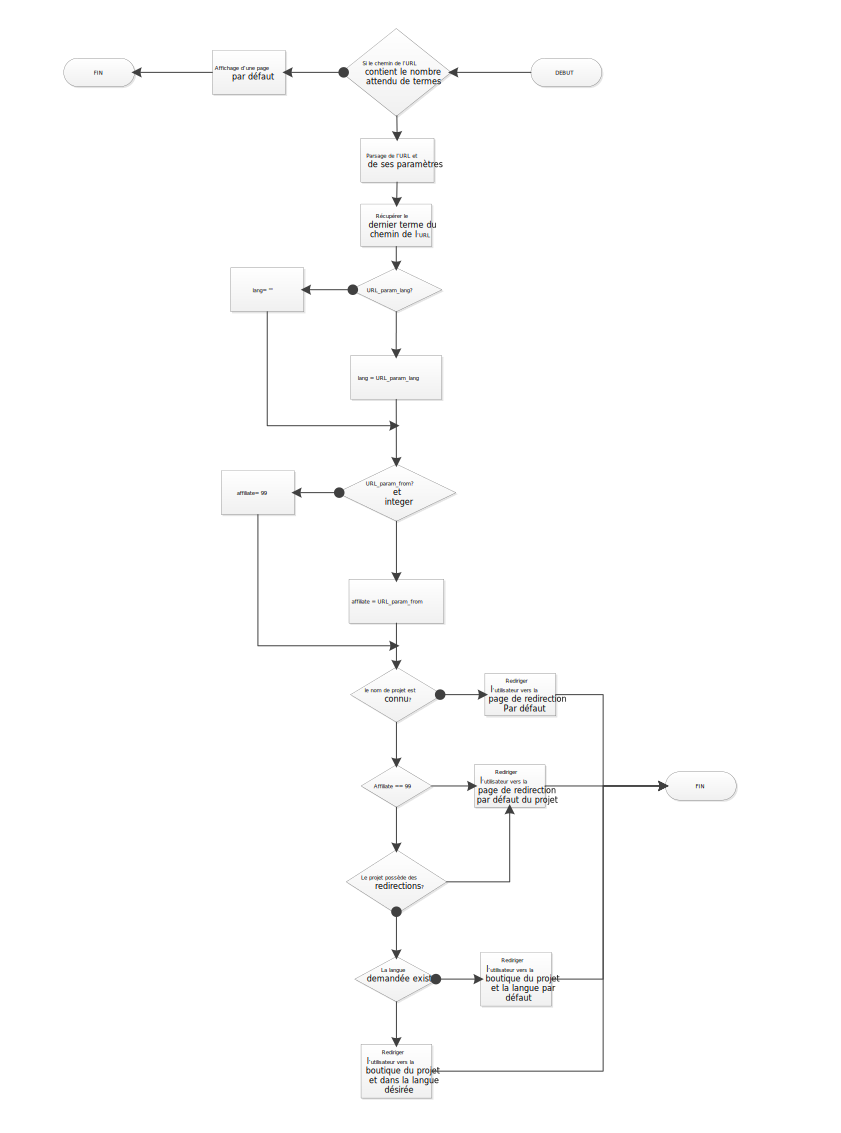
\includegraphics[scale=0.6]{images/redirection.png}
	\caption{Algorithme de redirection }
\end{figure}

\newpage

\subsubsection*{Récupération des données utilisateur}

Comme dit plus haut, la variable \textit{\textbf{environ}} passée en paramètre de la fonction \textit{application} nous permet de récupérer une somme d'information intéressante si celles-ci sont transmises par le navigateur client.

Les informations considérées comme ayant de l'importance pour nous sont:

\begin{itemize}
\item HTTP\_ACCEPT\_LANGUAGE : contient les différentes langues comprises par le navigateur client.
\item HTTP\_USER\_AGENT : permet de déterminer le navigateur (Chrom, Opéra, IE, Firefox, ...) ainsi que le système d'exploitation de l'utilisateur (Microsoft, Linux, IOS, Andorid, ...).
\item REMOTE\_ADDR : récupère l'ip du client, pour de la géolocalisation par exemple.
\end{itemize}

L'ensemble de ces informations si elles existent, dont en plus du nom du projet et du numéro de l'affilié sont transformés en un dictionnaire python. Par cette portion de code:

\begin{python}
#get interesting datas
datas = {
    "affiliate"        : affiliate,
    "project"          : projectName,
}
try:
    datas["prefered_language"] = environ["HTTP_ACCEPT_LANGUAGE"]
except KeyError:
    pass
try:
    datas["user_agent"]        = environ["HTTP_USER_AGENT"]
except KeyError:
    pass
try:
    datas["remote_ip"]         = environ["REMOTE_ADDR"]
except KeyError:
    pass
\end{python}


\subsection*{Transmission des données}

Si le projet n'est pas désactivé pour le tracking des données, il est possible d'envoyer les données par le moyen d'un socket et ce fourni par la librairie standard.

En début de lancement du script de redirection, le mod\_wsgi tente d'ouvrir un socket sur le port d'écoute choisi dans la configuration si le port n'accepte pas de connections l'erreur est écrite dans un fichier de log et le script effectue seulement les redirection mais ne réalise aucun enregistrement des données utilisateurs.

Dans le cas où la connexion avec le script a pu être établie, et si le projet concernée par la redirection est actif (cf:configuration des projets). Alors le transfert est réalisé par cette ligne de code:

\begin{python}
datas = cPickle.dumps(datas)
size = len(datas)
pattern = "{:0%d}"%8
dataSocket.sendall(pattern.format(size)+datas)
\end{python}

Ici datas correspond au dictionnaire de données à transmettre et la taille de l'header est définie à 8 caractères.

\newpage

\subsubsection*{Comment transmettre ces données}
Le choix d'avoir décider d'acheminer les données par socket python nous impose la transmission des information par chaîne de caractères. Pour ce faire il nous faut sérialiser les données contenu dans le dictionnaire. Nous avons décidé d'utiliser le module Pickle de la librairie standard et même ça version compilée cPickle qui est 25 \% plus rapide que son homologue pur Python. 

\underline{exemple}:
\begin{python}
>>>monDict = {"param1":"value1", "param2":42, "param3":["element1", 12, True]}
#une fois dumpée
>>>dump = cPickle.dumps(monDict)
#génère cette chaîne de caractère
>>>print dump
(dp1
S'param3'
p2
(lp3
S'element1'
p4
aI12
aI01
asS'param2'
p5
I42
sS'param1'
p6
S'value1'
p7
s.
#de même il est possible de retransfomer cette chaîne de caractères en dictionnaire
>>>print cPickle.loads(dump)
{'param3': ['element1', 12, True], 'param2': 42, 'param1': 'value1'}
\end{python}

Nous possédons désormais un moyen efficace pour effectuer les transactions entre les différents script.

Mais ceci n'est pas suffisant car il s'est avéré qu'a un très nombres de connections simultanées, le système d'exploitation FreeBSD contrairement à Microsoft, fusionnait les différents dictionnaire en une seule chaîne de caratère et non en plusieurs paquets de données comme c'est le cas sur Windows, il a donc fallut réaliser un protocole de transmission de données.

La taille et le nombre des paquets d'informations étant très variables et donc imprédictible côté réception.  Un problème se pose lorsque l'on désire dissocier les groupes de données entre eux.

Nous avons donc choisi de réserver un certains nombre de caractères pour indiquer la longueur de la chaîne de caractère contenant les données sérialisée

\begin{figure}[h!]
	\centering
	\includegraphics[scale=0.6]{images/noaprotocol.png}
	\caption{Structure de données transmise par socket}
\end{figure}


\newpage

\section*{Script d'insertion}

Celui-ci est composé de deux thread et d'une fonction permettant de générer un mail en cas d'alerte:

\begin{itemize}
\item un thread serveur écoutant sur un éventuel client de datas ou de commandes.
\item un thread s'occupant d'insérer les données en BDD.
\end{itemize}

\subsection*{Structure du serveur d'écoute}
Celui-ci se présente sous la forme la d'une boucle infinie, cette structure débute par select qui est un appel système qui prends en paramètre trois listes de socket:

\begin{itemize}
\item connexions entrantes : dans notre elle composée du socket de datas et du socket de commande
\item connexions sortantes
\item erreurs inexplicables en entrée ou en sortie
\end{itemize}

Le select renvoie en sortie si un évènement correspondant aux sockets contenu dans les listes est survenu, un tuple de trois liste contenant les sockets concernés par l'évènement. Sinon le select bloque la boucle évitant au script de vérifier périodiquement si l'évènement à eu lieu, en effet c'est le système d'exploitation qui effectue ce test.

Ensuite on vérifie quel socket à été réveiller et pour quelle raison, si le socket se trouve être celui de commande, on utilise la commande système \textit{accept} sur le socket ainsi réveiller cette méthode renvoie un autre socket contenant la connexion entre le client et le serveur. On ajoute ce socket à la liste des connexions entrantes ainsi qu'a une autre liste contenant tous les sockets de commandes actifs. De même si le socket activé s'avère être celui de datas on réalise les mêmes opérations a ceci prêt que l'on ajoute cette nouvelle connexion dans la liste des sockets de datas actifs, puis on retourne au select.

Si le socket n'est ni un socket de datas ni un socket de commande , c'est donc qu'il s'agit d'un socket généré par la méthode accept, il peut donc soit être de type \textit{datas}  soit de type \textit{cmd}. 

Pour le déterminer on vérifie l'existence de ce socket dans la liste des sockets de commandes actifs, si c'est le cas on récupère un paquet de donnée de longueur fixe grâce la méthode \textit{recv} du module \textbf{socket}, si aucune donnée valide n'a été transmise alors cela signifie que le client à simplement envoyer un signal SIGPIPE de fermeture de socket, il faut donc fermer le socket grâce à \textit{close}, puis supprimer cette connexion détruites des connexions entrantes ainsi que des sockets de commandes actifs. Si les datas sont valides au les traite on exécute l'ordre si possible et on revient au select en attente d'un nouvel évènement.

Si le socket réveillé n'était pas non plus de la commande, on vérifie par acquis de conscience que le socket est bien du type \textit{datas}, et de même si aucune donnée n'est transmise c'est donc le client (le script de redirection dans notre cas) a mis fin à la connexion, il faut donc là aussi fermer le socket, supprimer la connexion de la des connexions entrantes et enfin retirer la connexions des sockets de datas actifs. dans le cas contraire on les traite et on retourne au select.

\subsection*{Traitement de la commande}
Pour que données de commande il faut qu'il s'agisse d'un nombre, si ce n'est pas le cas on retourne au select.

Pour le moment seul deux ordres sont disponibles:

\begin{itemize}
	\item 0 : ceci correspond à l'ordre \textit{\textbf{stop}} qui permet de stopper le script en mettant à True une variable globale
	\item 1 : cet ordre \textit{\textbf{antispam}} permet en modifiant une variable globale de réactiver l'envoie de mail en cas d'erreur
\end{itemize}

\newpage
\begin{figure}[h!]
	\centering 
	\includegraphics[scale=0.6]{images/select.png}
	\caption{Structure du serveur d'écoute}
\end{figure}

\newpage

\section*{Traitement des données}


\subsection*{Cas de figures défavorables}

Pour rappel un paquet d'informations est constitué d'un header contenant la taille en nombre de caractères des données sérialisée ainsi que les données a proprement parler.

\begin{figure}[h!]
	\centering 
	\includegraphics[scale=0.6]{images/uncomplete_packet.png}
	\caption{Exemple de réception de paquet incomplet}
\end{figure}

\'{A} chaque appel de la fonction \textit{recv} sur le socket de datas nous lisons un nombre fixe de caractères, il peut donc arriver que les datas ne puissent pas tenir sur la zone de lecture courante et donc se retrouve tronquée. Il faut donc attendre la prochaine lecture afin de reconstituer la donnée dans son ensemble.

De la même manière il peut aussi arriver que l'header soit réparti entre deux lectures. Dans ce cas il est impossible de se prononcer quand à la longueur des données attendues, il faut là aussi attendre un prochain train d'information pour prendre une décision.

\begin{figure}[h!]
	\centering 
	\includegraphics[scale=0.6]{images/uncomplete_header.png}
	\caption{Exemple de réception d'header incomplet}
\end{figure}
\newpage
\subsection*{Algorithme de lecture}

Toutes données reçues par le socket de datas est transmis à un buffer de chaîne de caractères. Tant que la longueur de ce buffer est supérieur à la longueur d'un header et donc que l'on est capable de déterminer la taille d'une donnée à attendre, ce annulant l'hypothèse de la figure 6. On applique cette algorithme:

\begin{figure}[h!]
	\centering 
	\includegraphics[scale=0.6]{images/datas_gathering.png}
	\caption{Algorithme de lecture de données transmises}
\end{figure}

\subsection*{Désérialisation}

Par sécurité, si la désérialisation des données échoue on purge les données car on ne peut pas déterminer à quel moment l'erreur est apparue.

Si aucun problème n'est survenu, le dictionnaire obtenu est ajouté à une FIFO commune aux threads de select et d'insertion en BDD.

\newpage

\section*{Stockage des données}
\subsection*{Moteur de BDD}
Un moteur de base de données est l'ensemble des différents mécanismes permettant la manipulations des informations stockées. 

\subsection*{Deux prétendants}

Les moteurs les plus utilisés sur les serveurs MySQL se nomment:

\begin{itemize}
	\item{MyISAM} 
	\item{InnoDB} 
\end{itemize}

Pour tester les performances de ces deux moteurs, réalisons une série de 100000 insertions de 6 champs chacun. Cette expérience nous présente le résultat suivant:
  
\begin{figure}[h]
	\centering
	\begin{subfigure}[b]{0.6\textwidth}
		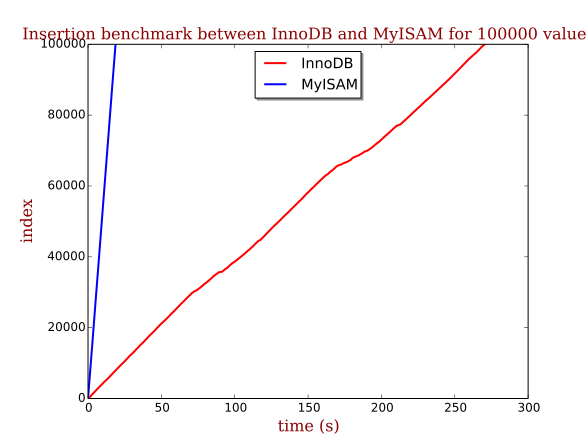
\includegraphics[width=\textwidth]{images/benchmark_inno_isam_100000.png}
	\end{subfigure}
	\begin{subfigure}[b]{0.3\textwidth}
		\begin{tabular}{|c|c|}
		\hline Engine & inserts.s $^{-1}$ \\ 
		\hline InnoDB & 404 \\ 
		\hline MyISAM & 5479 \\ 
		\hline 
		\end{tabular} 
	\end{subfigure}
\end{figure}

On remarque que le moteur InnoDB est plus de 13.5 fois plus lent que MyISAN pour effectuer la même opération.

Ceci est dû au fait que le moteur InnoDB est ce que l'on nomme transactionnel. Pour rappel une transaction est une séquence de commande qui commence par un BEGIN, continue par des opération CRUD (SELECT, INSERT, UPDATE, DELETE) et fini soit par un COMMIT qui valide les opérations précédente soit par un ROLLBACK qui les annulent. Contrairement à MyISAM qui se contente des opérations CRUD.

Mais la vitesse d'insertion n'est pas l'unique condition de choix. En effet nous désirons aussi une sécurité sur l'insertion des données, ce qui nous est permis grâce au système de transaction qui en cas d'erreur permet d'annuler l'insertion et de ne pas compromettre les données.

De plus InnoDB semblent tout à fait capable d'assurer les 100 insertions par secondes requis. Nous utiliserons donc ce moteur pour la table qui contiendra les données utilisateur.

\subsection*{Gérer les problèmes de communication avec la BDD}

Les erreurs d'enregistrement peuvent être provoquées par des problèmes temporaires comme de la latence sur la ligne ou un redémarrage du serveur contenant la base de données.
Nous avons donc besoin d'un moyen de pouvoir nous reconnecter en cas de déconnexion non désiré. Pour se faire nous avons décidé d'utiliser le connecteur mysql développé par Oracle "python mysql connector" celui-ci permet en effet se reconnecter à base de données

\subsection*{Stockage des données}

L'insertion des données est effectuée dans un thread infini retardé par un sleep de 0.001 seconde afin de ménager le temps processeur. A chaque tour de boucle on vérifie si la FIFO commune au 2 threads n'est pas vide, si ce n'est pas le cas alors on dépile un élément, celui-ci est bien évidemment le dictionnaire généré par le script de redirection lors du passage d'un utilisateur, afin de l'horodaté on rajoute une clef "date"  puis on essaie 3 fois d'insérer les données. Si cela échoue les deux premières fois on effectue un rollback de la transaction on rempile le dictionnaire dans la FIFO, puis on attends 5 secondes avant de réessayer, au bout de 3 essais on abandonne définitivement et on envoie un mail. Si tout c'est bien passé on commit la transaction.

\section*{Gestion de la configuration}

Comme évoqué pour la gestion des redirections des projets, l'ensemble de la configuration est géré par un fichier XML, il est structuré en deux parties:

\begin{itemize}
	\item{La configuration des scripts} 
	\item{La configurations des projets} 
\end{itemize}


